
\subsection{Reference Implementation}

Before implementing a code generator one has to know what the target code is. Therefore a reference implementation has been
developed which was coded to large degree manually. From this reference code the templates can be derived. Also this is a
manual step.
\begin{wrapfigure}[24]{l}{0.48\textwidth}
 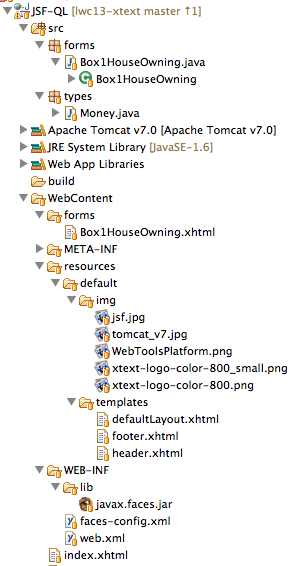
\includegraphics[width=9cm]{./images/chapter02/referenceimpl_projecttree.png}
\end{wrapfigure}
We use a Java Server Faces (JSF) based application, which can be deployed on any
Java Web container (also known as a Servlet container) like Glassfish, JBoss and Apache Tomcat.

The screenshot shows the structure of the web application project. The application is available for download from the project 
homepage (\href{http://lwc13-xtext.eclipselabs.org.codespot.com/files/JSF-QL-1.0.zip}{JSF-QL-1.0.zip})
 
Large parts of the application are not derivable from the model, they build the skeleton of the project. This is:
\begin{itemize}
\item Custom types (\texttt{src/types/*})
\item Custom type converter (\texttt{src/converter/*})
\item Libraries \newline (\texttt{WebContent/WEB-INF/lib/*})
\item Web Application Descriptor \newline (\texttt{WebContent/WEB-INF/web.xml})
\item Faces configuration \newline
(\texttt{WebContent/WEB-INF/faces-config.xml})
\item Images \newline (\texttt{WebContent/resources/default/img/*})
\item Page Templates \newline
(\texttt{WebContent/resources/default/templates/*})
\end{itemize} 

After describing some necessary configuration of the IDE we will focus on the
parts which are dependent on the QL model and thus subject of code generation
in sub sesction \ref{subsec:referenceForms}.
These artifacts are:
\begin{itemize}
\item Java Bean classes representing the state of a Form (\texttt{src/forms})
\item JSF enabled XHTML pages representing the presentation of a Form (\texttt{WebContent/forms/*})
\end{itemize}

\subsubsection{General}
\label{subsec:referenceGeneral}
Root entry of the web application is the \texttt{welcome-file}
\texttt{WebContent/index.xhtml} declared in \texttt{WebContent/WEB-INF/web.xml}.

The \texttt{index.xhtml} within \texttt{WebContent/} will be helpful to
integrate the generated forms into the whole web application by use of JSF xhtml
templating later.
\footnote{\url{http://docs.oracle.com/javaee/6/javaserverfaces/2.1/docs/vdldocs/facelets/}}
 
This file implements the main composition of the applications layout and
pages. The main layout is provided by a default template placed in
\texttt{WebContent/resources/default/templates/defaultLayout.xhtml}.

\begin{lstlisting}[language=HTML]
<?xml version='1.0' encoding='UTF-8' ?>
<!DOCTYPE html PUBLIC "-//W3C//DTD XHTML 1.0 Transitional//EN" 
    "http://www.w3.org/TR/xhtml1/DTD/xhtml1-transitional.dtd">
<html xmlns="http://www.w3.org/1999/xhtml"
  xmlns:h="http://java.sun.com/jsf/html"
  xmlns:ui="http://java.sun.com/jsf/facelets">
<body>

  <ui:composition
    template="/resources/default/templates/defaultLayout.xhtml">
    <ui:define name="content">
      Hello World!
    </ui:define>
  </ui:composition>

</body>

</html>
\end{lstlisting}

To change the layout it is just necesarry to change the main layout reference in
the attribute \texttt{template} of the \texttt{facelets:composite} component.
The current web application urgently needs a defined facelets:insert section
with name 'content' for proper composition which is declared in
\texttt{/resources/default/templates/defaultLayout.xhtml}.

\begin{lstlisting}[language=HTML]
 <ui:insert name="content">
    	Content area. Compose by use of <facelet:define name="content">.
  </ui:insert>
\end{lstlisting}

Subpages of the application should use the main index.xhtml itself as
their template and overwrite the content section with custom output by the same
pattern.

\begin{lstlisting}[language=HTML] 
	<ui:composition template="/index.xhtml">
  		<ui:define name="content">
  		...
  		</ui:define>
 	</ui:composition>
\end{lstlisting}

\subsubsection{IDE Configuration}

\paragraph{Webtools}
yxcvyxcvyxcvyxvc
\paragraph{Install Tomcat}
xycvyxcvyxcvyxcv

\subsubsection{Import and run reference}
xyvxcvyxcvyxcvyxcv

\subsubsection{Reference Forms}
\label{subsec:referenceForms}
general (eg index.xhtml)

\paragraph{Bean}
yxcvyxcvyxcvyxcvyxcv

\paragraph{Form}
yxcvyxcvyxcvyxcvxycv



